\documentclass[11pt,a4paper]{article}
\usepackage[margin=1in]{geometry}
\usepackage{url}
\usepackage{hyperref}
\usepackage{paralist} % For use with \begin{compactitem}... or \begin{compactenum}
\usepackage{microtype}		% For decreasing the hyphenation frequency
\microtypesetup{activate=true}
\usepackage{xcolor}
\usepackage{placeins}
\usepackage{graphicx}

\makeatletter
\def\ps@pprintTitle{%
  \let\@oddhead\@empty
  \let\@evenhead\@empty
  \def\@oddfoot{\reset@font\hfil\thepage\hfil}
  \let\@evenfoot\@oddfoot
}
\makeatother


\begin{document}
%\begin{frontmatter}

\begin{titlepage}
	\clearpage\thispagestyle{empty}
	\centering
	\vspace{1cm}
		
	\rule{\linewidth}{1mm} \\[0.5cm]
	{ \Large \bfseries ISyE 6740 - Summer 2023\\[0.2cm]
		Project Report}\\[0.5cm]
	\rule{\linewidth}{1mm} \\[1cm]

		\begin{tabular}{l p{5cm}}
		\textbf{Team Member Names:} Vivi Banh (Proposal, Final Report, and Model Evaluation) \\ \& Chukwuemeka Okoli (Proposal, Final Report, and Model Development) \\[10pt]
		\textbf{Project Title:} Deep Neural Network for Shoe Model Identification  \\[10pt]
		%\textbf{Please include (at least) the following sections.} & \\
		\end{tabular} 

\end{titlepage}	
%\end{frontmatter}
	

\section{Problem Statement}\label{sec1}
In today's fashion-forward society, social media plays a pivotal role in shaping consumer habits and driving trends. As people browse through fashion photos online, they seek convenient ways to identify and purchase the products showcased in those images. However, traditional methods of searching for unknown products on search engines can be frustrating and time-consuming.  \\

\noindent
Our project aims to develop an image classification system for shoe classes worn by models in photos. The system will accurately identify the class of shoes in images and provide users with the corresponding class information. This will streamline the shopping experience, making it easier for consumers to find and purchase specific shoe models they are interested in.\\

\noindent
Integrating our image classification system into popular platforms like Instagram or a web application can bring significant benefits to retailers and e-commerce platforms. By seamlessly incorporating a product identification feature, businesses can captivate potential buyers, enhance customer engagement, and drive conversions. This transformative capability bridges the gap between inspiration and purchase, transforming social media platforms into highly effective sales channels. The integration of our image classification system can create new opportunities for both retailers and consumers, maximizing sales potential and delivering an exceptional shopping experience. 
	
\section{Data Source} 
The data utilized for this project is the UT Zappos50K Shoe Dataset (ver 1.2), curated by Yu and Grauman (2014) and available on Kaggle.com. This comprehensive shoe dataset comprises 50,025 catalog images obtained from Zappos.com. The images have dimensions of 136 x 102 pixels, showcasing shoes centered on a white background and consistently oriented for ease of analysis. The dataset encompasses various shoe models. The classes to predict include 20 different class of shoes. We trained a neural network and evaluate the performance of our trained model.  
		
\section{Methodology} 
Our problem is a classification problem since we are trying to determine the category of shoe or class of shoe from an image of several shoes from different brand names. We utilized a Convolutional Neural Network (CNN) model, a deep learning architecture well-suited for image classification tasks. The CNN model is trained using the labeled shoe images to learn the distinctive features of each shoe model. We built a custom Convolutional Neural Network (CNN) architecture with three convolutional blocks, followed by a classifier head with two dense layers as the starting model. The model uses the Keras Sequential API to create the architecture.

\subsection{Data Preprocessing}
The preprocessing steps we applied including resizing and normalization, to ensure they are in a suitable format for training. Data augmentation techniques such as vertical and horizontal reflections, rotation up to 90 degrees, and vertical and horizontal shifting of the images up to 20\% of their original size will be applied to enhance the model's ability to generalize.  To preprocess the image, we used the MobileNet V2 preprocessing function from Keras API.  To load the images from disk in small batches of size 32, we used an ``ImageDataGenerator``.  We resized the images and used a small images of size 224 * 224. We have 20 classes namely ``Ankle Boots'', ``Knee High Boots'', ``Over the Knee Boots'', ``Prewalker Boots'', ``Mid-Calf Boots'', ``Athletic Sandals'', ``Flat Sandals'', ``Heel Sandals'', ``Boat Shoes'', ``Flats Shoes'', ``Oxfords Shoes'', ``Clogs and Mules Shoes'',  ``Firstwalker Shoes'', ``Sneakers and Athletic Shoes'', ``Heels Shoes'', ``Prewalker Shoes'', ``Crib Shoes'', ``Loafers Shoes'', ``Slipper Heels Slippers'', ``Slipper Flats Slippers'', ``Boot Slippers''. The generator used the folder structure where the images were stored to infer the labels for the images. We split the data into training, validation and testing sets with 70\% of the data for training the model, 15\% for validating the datasetand selecting the best parameters, and 15\% for testing the model. 

\subsection{Model Architecture}
The neural network is organized in layers meaning we take an image of a shoe, pass it through all the layers and get a prediction of what class the shoe belongs too. We used a custom CNN architecture with three convolutional blocks, followed by a classifier head with two dense layers. The convolutional layer consists of many filters giving us multiple feature maps for each filter.  The output of one convolutional layer is used as input into the next layer. The structure of the neural network is shown in \textbf{Fig. \ref{neural_network}} below:

 \begin{figure}[h!]
\centering
  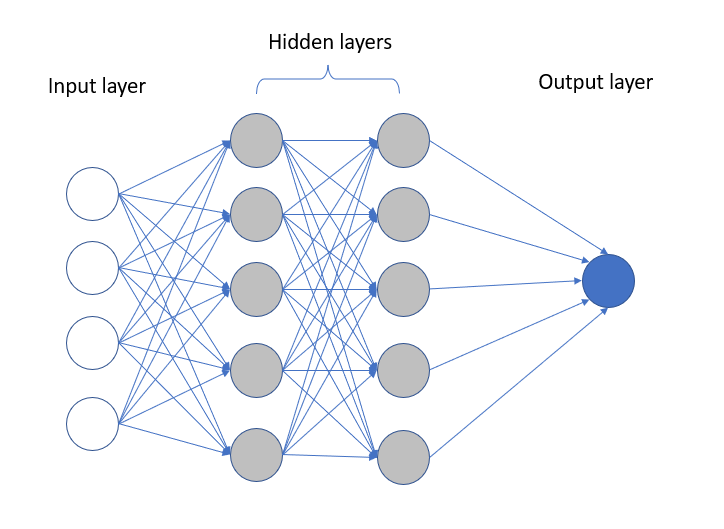
\includegraphics[width=0.75\linewidth]{neural network.png}
  \caption{Structure of a neural network}
  \label{neural_network}
\end{figure}

\subsection{Model Development}
The CNN model is used to train labeled shoe images as input and their corresponding shoe model names as target labels. The model learnt to recognize the visual patterns associated with each shoe model during the training process.  To develop the model, we used \emph{Conv2D} as input layer with the first convolutional block followed by a \emph{MaxPooling2D} layer. The MaxPooling2D layer reduces the spatial dimensions of the output by performing max-pooling operation. The second convolutional block is similar to the first one, with 64 filters and a kernel size of 3x3. Again, a MaxPooling2D layer follows the Conv2D layer to reduce spatial dimensions. The third convolutional block is similar to the previous ones, with 128 filters and a kernel size of 3x3. Another MaxPooling2D layer follows the Conv2D layer. After the last MaxPooling2D layer, a Flatten layer is used to convert the 2D feature maps into a 1D vector, which is then fed into the fully connected layers. A Dense layer with 740 units and ReLU activation function is used. Finally, there is another Dense layer with 20 units and a softmax activation function.  

This is the output layer, and it represents the probability distribution over the 20 classes in the classification task. The chosen optimizer is ``adam," which is a popular adaptive learning rate optimization algorithm. The loss function used is ``categorical\_crossentropy," which is appropriate for multi-class classification problems with one-hot encoded labels. The model is evaluated based on the "accuracy" metric during training and testing. A schematic of the convolutional neural network developed is shown in \textbf{Fig. \ref{schema}}.

 \begin{figure}[h!]
 \centering
  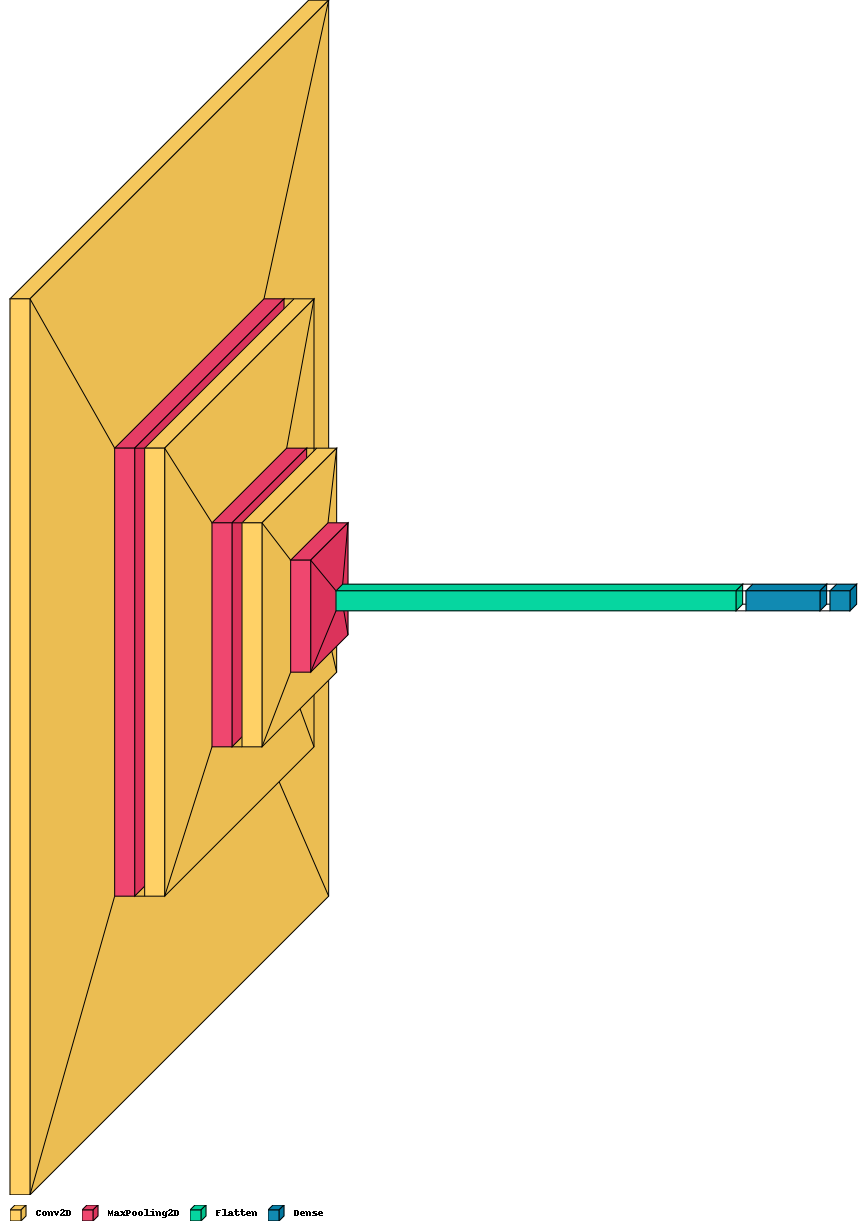
\includegraphics[width=0.85\linewidth]{schema.png}
  \caption{A schematic of the convolutional neural network}
  \label{schema}
\end{figure}

\noindent
In the Adam optimization algorithm, we specify the learning rate, which determines how fast our network learns. We set a reasonable value of $0.01$ since if we set it too high, the network learns too fast and skip some details. If it is too low, then the model training time increases significantly.We define the loss function as ``CategoricalCrossentropy'' which is usually used to train a classification model with multiple classes. We chose accuracy as our metric since we want to determine the percentage of correct classification that the model achieves. We specify the \emph{epoch} which is the number of times the model run through the training data. We set a value of $10$ since using more epoch means the model learns the training data better. We don't want the value to be too high or the model starts to overfit the training data. 

\section{Evaluation and Final Results} 
The plot of the loss and accuracy on the dataset is shown in Figure \ref{cnn_loss}. As observed, there is a notable difference between the training accuracy and validation accuracy, indicating the presence of overfitting. The model achieved a high training accuracy of 98.84\% but a lower validation accuracy of 82.84%.

To address the issue of overfitting and improve the model's overall performance, we applied two techniques: data augmentation and dropout.

1. Data Augmentation:
   Data augmentation is a technique that involves generating additional training data by applying various transformations to the existing images. These transformations include flipping, rotation, shifting, and zooming. By augmenting the dataset with these variations, we introduce more diversity and variations to the training data, which helps the model generalize better to unseen images.

2. Dropout:
   Dropout is a regularization technique that aims to reduce overfitting by randomly setting a fraction of the output units (neurons) to zero during training. This means that during each training iteration, a certain percentage of neurons are "dropped out" or deactivated, forcing the model to learn redundant representations and preventing complex co-adaptations between neurons. Dropout acts as a form of ensemble learning, as it trains multiple sub-networks with different combinations of neurons active and then averages their predictions during inference.

By adding data augmentation and dropout to the model, we observed a reduction in overfitting, and the gap between the training and validation accuracies was narrowed. The dropout value used in the model was set to 0.2, meaning 20\% of the output units from the layer were randomly dropped out during training.

The schematic of the Convolutional Neural Network with dropout is depicted in Figure \ref{dropout_schema}. This updated model with data augmentation and dropout shows improved generalization capabilities and better performance on unseen data.

\begin{figure}[htbp]
  \centering
  % Include the plot here using \includegraphics
  \caption{Plot of Loss and Accuracy on the Dataset}
  \label{cnn_loss}
\end{figure}

\begin{figure}[htbp]
  \centering
  % Include the dropout schematic here using \includegraphics
  \caption{Schematic of Convolutional Neural Network with Dropout}
  \label{dropout_schema}
\end{figure}

 \begin{figure}[h!]
 \centering
  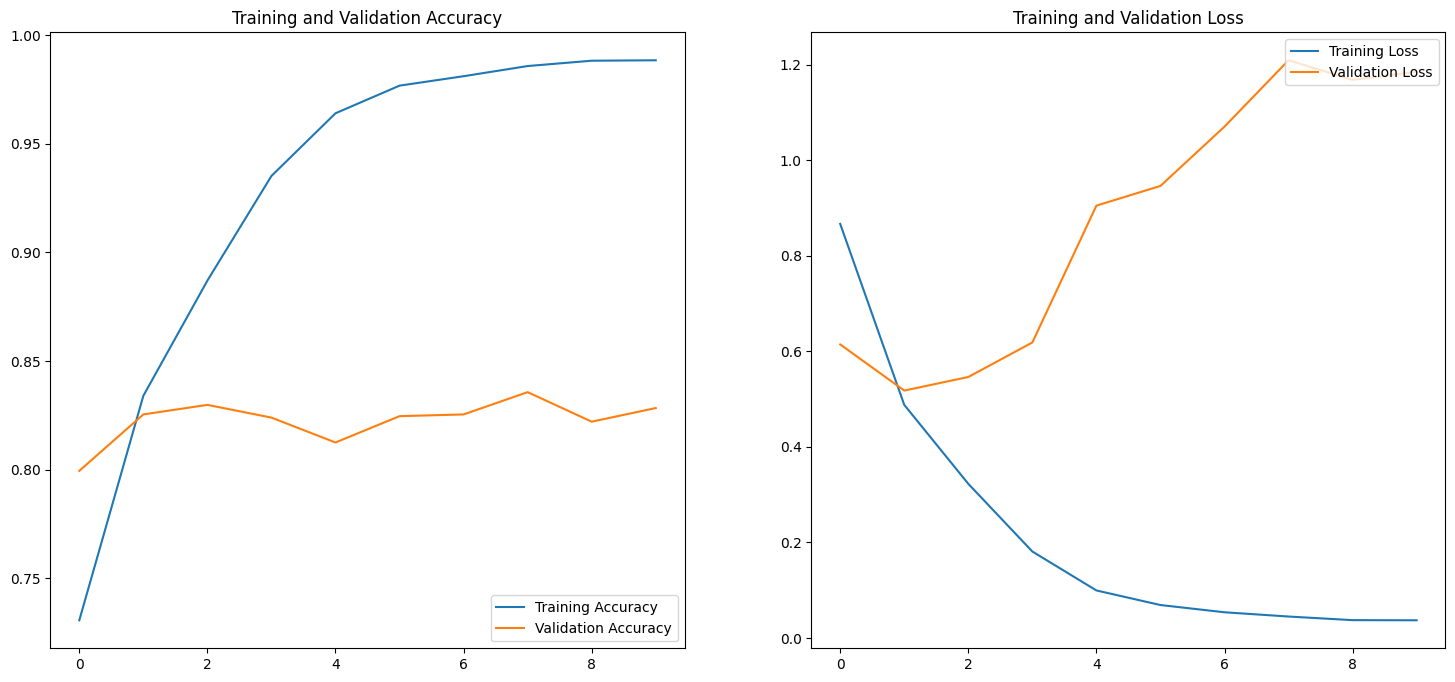
\includegraphics[width=\linewidth]{training_valid_plot.png}
  \caption{The plot of loss and accuracy on train dataset}
  \label{cnn_loss}
\end{figure}

 \begin{figure}[h!]
 \centering
  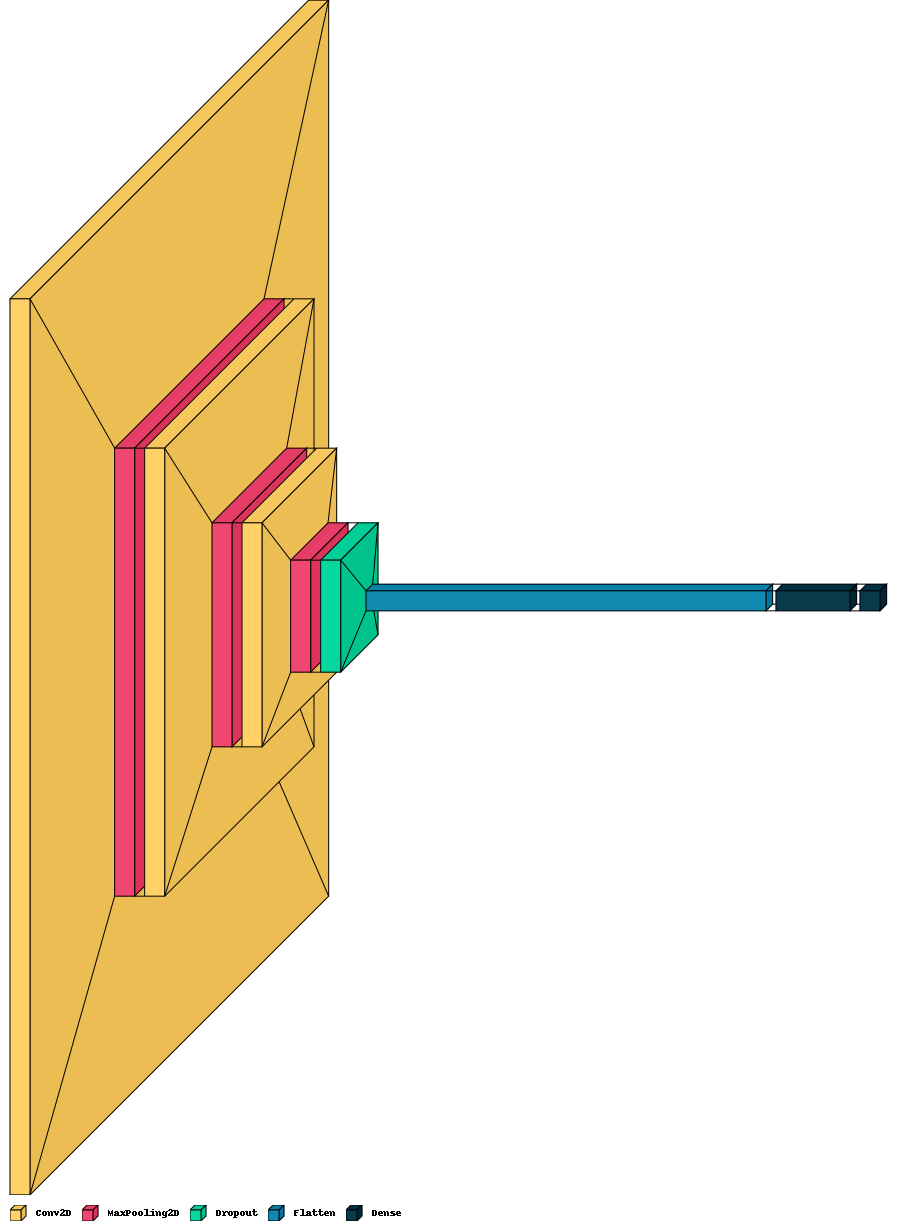
\includegraphics[width=0.85\linewidth]{dropout_schema.png}
  \caption{A schematic of the convolutional neural network with dropout}
  \label{dropout_schema}
\end{figure}


 \begin{figure}[h!]
 \centering
  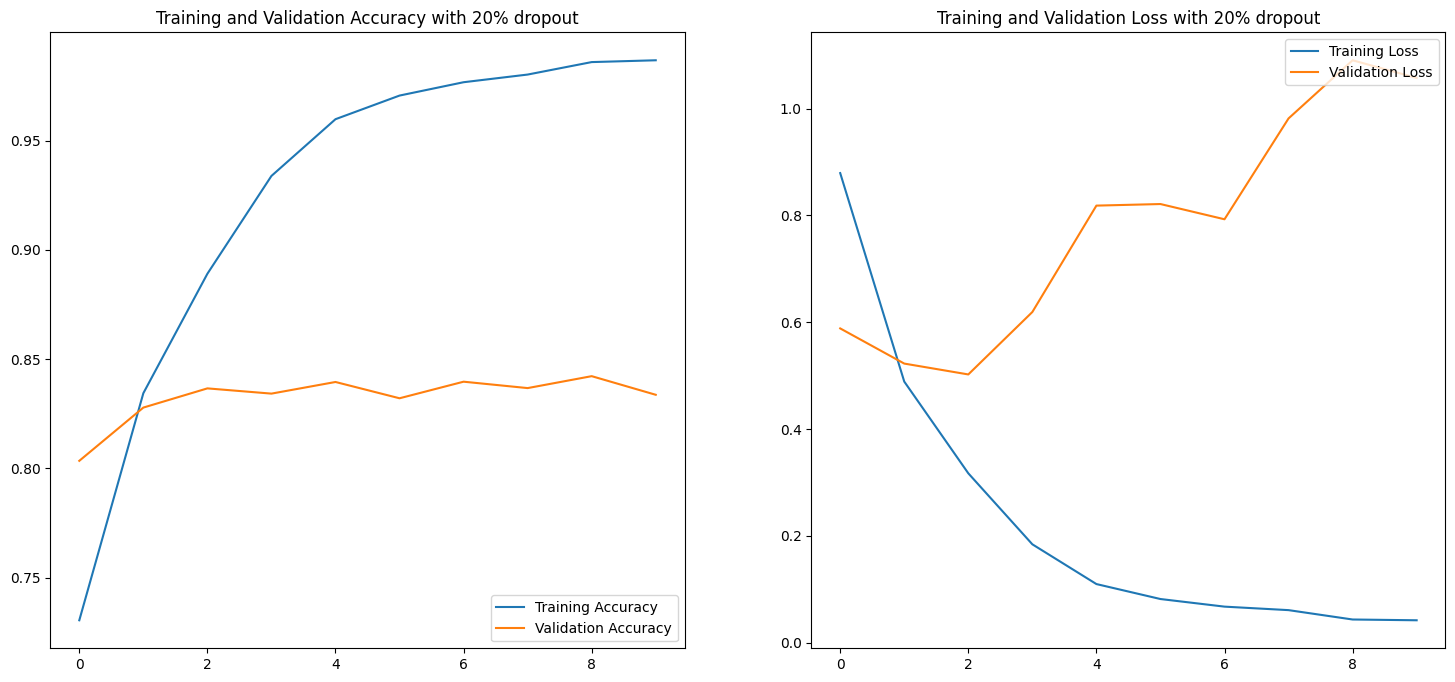
\includegraphics[width=\linewidth]{dropout_training_plot.png}
  \caption{The plot of loss and accuracy on train dataset with dropout}
  \label{dropout_training}
\end{figure}
\FloatBarrier

% Please add the following required packages to your document preamble:
% \usepackage{graphicx}
\begin{table}[h!]
\centering
\resizebox{\textwidth}{!}{%
\begin{tabular}{lcccccccccc} \hline
\begin{tabular}{lcccccccccc} \hline
Model Before Dropout
Epoch               & 1      & 2      & 3      & 4      & 5      & 6      & 7      & 8      & 9      & 10     \\
Loss                & 0.8665 & 0.4879 & 0.3227 & 0.1810 & 0.0996 & 0.0690 & 0.0539 & 0.0450 & 0.0374 & 0.0371 \\
Train accuracy      & 0.7307 & 0.8340 & 0.8870 & 0.9352 & 0.9640 & 0.9768 & 0.9811 & 0.9858 & 0.9882 & 0.9884 \\
Validation accuracy & 0.7995 & 0.8254 & 0.8298 & 0.8240 & 0.8125 & 0.8246 & 0.8254 & 0.8357 & 0.8221 & 0.8284 \\ \hline
\end{tabular}%
}
\caption{Result of Model Training and Validation Accuracy with Epochs}
\label{tab:train_loss}
\end{table}

The plot of loss and accuracy on the training dataset with dropout is depicted in Figure \ref{dropout_training}. After training the model with dropout, we proceeded to make predictions on the test dataset to evaluate its performance. We used accuracy as the metric to assess how well the model performed.

Before removing dropout, the model achieved an accuracy of 81.59\% on the test dataset. However, after removing 20\% dropout, the model's accuracy did not show any significant increase, reaching 98.68\%. On the other hand, the validation accuracy increased to 83.37\%, indicating that adding dropout did not lead to a noticeable improvement in model prediction.

One possible reason for not observing a significant improvement is that the original model already had a robust performance, and the dropout regularization might not have contributed significantly to its generalization. Additionally, with a large dataset and effective data augmentation techniques, the model might have been less prone to overfitting, making the impact of dropout less prominent.

Both models, with and without dropout, show the expected behavior during training: as the number of epochs increases, the loss decreases, and accuracy increases. This behavior is typical in the learning process of neural networks.

In conclusion, while dropout is a powerful regularization technique to control overfitting, its impact on the already well-performing model might not be as pronounced. The model's high accuracy on the test dataset indicates its effectiveness in correctly classifying shoe images. Adding dropout in this case might not have been essential to further improve the model's predictive performance.

% Please add the following required packages to your document preamble:
% \usepackage{graphicx}
\begin{table}[h!]
\centering
\resizebox{\textwidth}{!}{%
\begin{tabular}{lcccccccccc} \hline
Model After Dropout
Epoch               & 1      & 2      & 3      & 4      & 5      & 6      & 7      & 8      & 9      & 10     \\
Loss                & 0.8791 & 0.4889 & 0.3172 & 0.1843 & 0.1099 & 0.0819 & 0.0676 & 0.0611 & 0.0435 & 0.0421 \\
Train accuracy      & 0.7305 & 0.8344 & 0.8891 & 0.9339 & 0.9598 & 0.9706 & 0.9767 & 0.9803 & 0.9860 & 0.9868 \\
Validation accuracy & 0.8035 & 0.8278 & 0.8366 & 0.8342 & 0.8395 & 0.8321 & 0.8397 & 0.8368 & 0.8422 & 0.8337 \\ \hline
\end{tabular}%
}
\caption{Result of Model Training and Validation Accuracy After Dropout with Epochs}
\label{tab:dropout_train_loss}
\end{table}

Using the trained model, we tested the model on the test dataset and perform inference on a sample of images.nThe prediction on the test set gave an accuracy of 82.7\%. The final model developed was a well-trained model capable of accurately identifying shoe worn from shoe image. 


The success of the project will be determined by the model's ability to achieve a high level of accuracy in identifying the correct shoe models from the images, providing a solid foundation for further advancements in image classification and consumer-driven shopping experiences. 


\section{Conclusion}
For future enhancements, the trained model can be deployed as a user-facing application to enable a user-friendly experience. Consumers will be able to upload images and receive the corresponding shoe model names as the output. This application will streamline the process of identifying and purchasing specific shoe models, enhancing the shopping experience for consumers. One thing we didn't try out was to compare the performance of our trained model with other pre-trained model like ResNet50 and Fastai models.

\pagebreak
\section{References} 
		\begin{enumerate}
		\item Albawi, S., Mohammed, T. A., \& Al-Zawi, S. (2017). Understanding of a Convolutional Neural Network. 2017 International Conference on Engineering and Technology (ICET), 1–6. https://doi.org/10.1109/icengtechnol.2017.8308186  
		\item Sharma, N., Jain, V., \& Mishra, A. (2018). An Analysis Of Convolutional Neural Networks For Image Classification. Procedia Computer Science, 132, 377–384. https://doi.org/10.1016/j.procs.2018.05.198
		\item Yu, A., \& Grauman, K. (2014). Fine-Grained Visual Comparisons with Local Learning. Computer Vision and Pattern Recognition. https://doi.org/10.1109/cvpr.2014.32 
		\end{enumerate}
\end{document}